% https://piped.video/watch?v=rx7wwtmFlD8
% arara: pdflatex: { shell: yes } until !found('log', '\\(?(R|r)e\\)?run (to get|LaTeX)')
\documentclass[a4paper,
	DIV=13,
	14pt,
	BCOR=10mm,
	department=FakEI,
	% lucida,
	% KeepRoman,
	twoside,
	parskip=half,
	automark,
	aspectratio=169
	% headsepline,
]{beamer}
\usetheme{Copenhagen}

\setbeamertemplate{navigation symbols}{} % hide bottom page navigation
% \setbeamercovered{transparent} % transparent see next slide (when part of frame)
\setbeamertemplate{headline}{} % hide section navigation

\usepackage[utf8]{inputenc}

% \usepackage[english]{babel}
\usepackage[ngerman]{babel}

\usepackage{float}

% clickable toc, citations
\usepackage{hyperref}
\hypersetup{
	colorlinks,
	citecolor=black,
	filecolor=black,
	linkcolor=black,
	urlcolor=black
}

\date{\today}

% \pagestyle{headings}

\usepackage{lipsum}

\title{Warum jeder Programmieren lernen sollte}

\author{Jakob Pistohl \\ 3333475}

\date{19. April 2024}

\begin{document}

\maketitle

\section{Warum jeder Programmieren lernen sollte}
\begin{frame}{Warum jeder Programmieren lernen sollte}
	\begin{columns}
		\column{0.7\textwidth}
		\begin{itemize}
			\item<2-> Jeder sollte wissen, was möglich ist
			\item<3-> Es kann sehr viel Zeit gespart werden
			\item<4-> Es ist gar nicht so kompliziert
		\end{itemize}
		\column{0.4\textwidth}
		\begin{figure}[H]
			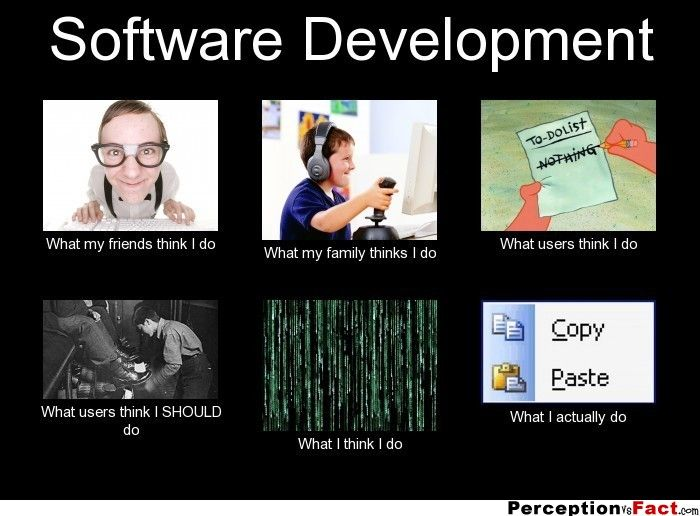
\includegraphics[width=\linewidth]{img/What-they-think.jpg}<4->
		\end{figure}
	\end{columns}
\end{frame}

\section{Python}
\begin{frame}{Python}
	\begin{columns}
		\column{0.7\textwidth}
		\begin{itemize}
			\item Funktioniert auf allen Systemen
			\item Anfängerfreundlich
			\item Viele öffentliche Ressourcen
		\end{itemize}
		\column{0.4\textwidth}
		\begin{figure}[H]
			
\includegraphics[width=\linewidth]{img/python.png}
		\end{figure}
	\end{columns}
\end{frame}

\section{QR-Code}
\begin{frame}{QR-Code}
\end{frame}

\begin{frame}{QR-Code}
	\begin{figure}[H]
		
\includegraphics[width=0.8\linewidth]{img/ChatGPT.png}
	\end{figure}
\end{frame}

\begin{frame}{QR-Code}
	\begin{figure}[H]
		
\includegraphics[width=\linewidth]{img/ChatGPT-code-Q.png}
	\end{figure}
\end{frame}

\begin{frame}{QR-Code}
	\begin{columns}
		\column{0.5\textwidth}
		\begin{figure}[H]
			
\includegraphics[width=\linewidth]{img/ChatGPT-code-Q.png}
		\end{figure}

		\column{0.5\textwidth}
		\begin{figure}[H]
			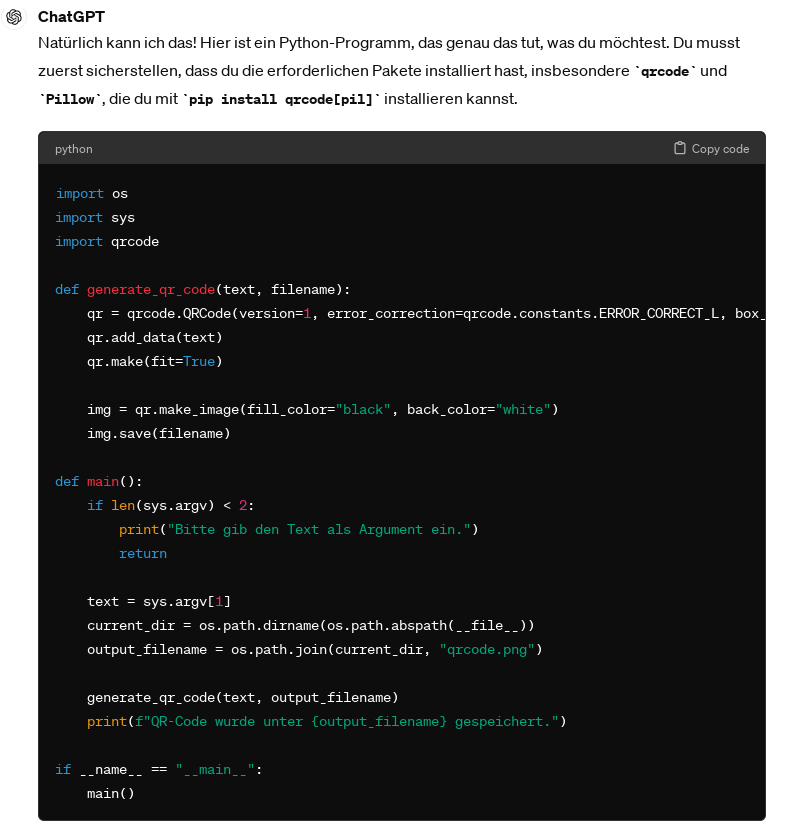
\includegraphics[height=0.8\textheight]{img/ChatGPT-code-A.png}
		\end{figure}
	\end{columns}
\end{frame}

\begin{frame}{QR-Code Fehler}
	\begin{figure}[H]
		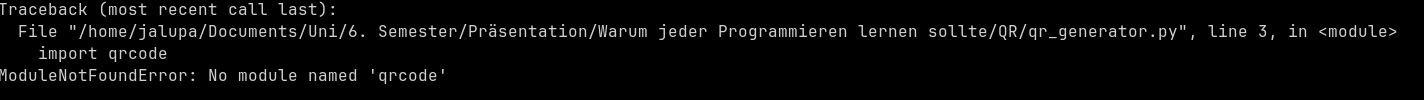
\includegraphics[width=\linewidth]{img/Error.png}
	\end{figure}
	\begin{figure}[H]
		
\includegraphics[width=\linewidth]{img/ChatGPT-error-Q.png}<2->
	\end{figure}
\end{frame}

\begin{frame}{QR-Code}
	\begin{columns}
		\column{0.5\textwidth}
		\begin{figure}[H]
			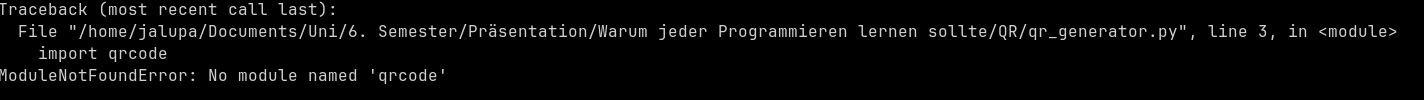
\includegraphics[width=\linewidth]{img/Error.png}
		\end{figure}

		\begin{figure}[H]
			
\includegraphics[width=\linewidth]{img/ChatGPT-error-Q.png}
		\end{figure}

		\column{0.5\textwidth}
		\begin{figure}[H]
			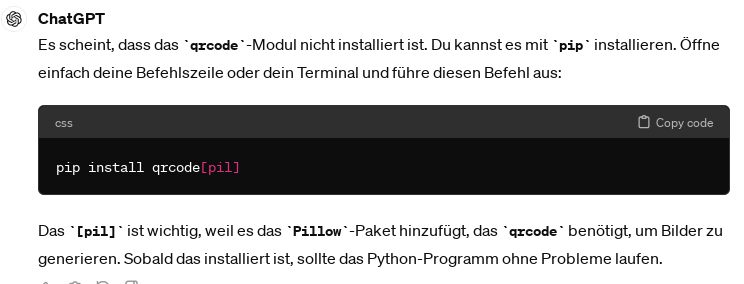
\includegraphics[width=\linewidth]{img/ChatGPT-error-A.png}
		\end{figure}
	\end{columns}
\end{frame}

\section{Wasserzeichen}
\begin{frame}{Wasserzeichen}
	\begin{columns}
		\column{0.5\textwidth}<2->
		\begin{figure}[H]
			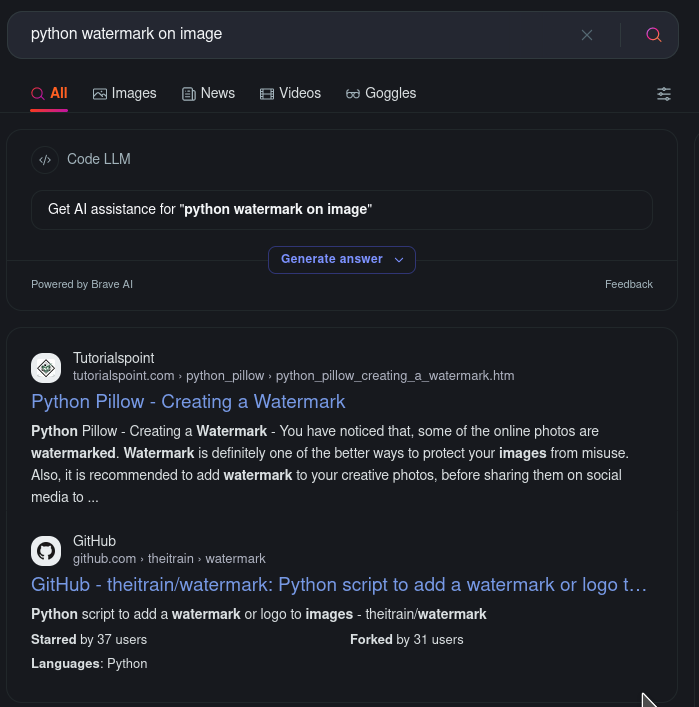
\includegraphics[height=0.8\textheight]{img/first-search.png}
		\end{figure}

		\column{0.5\textwidth}<3->
		\begin{figure}[H]
			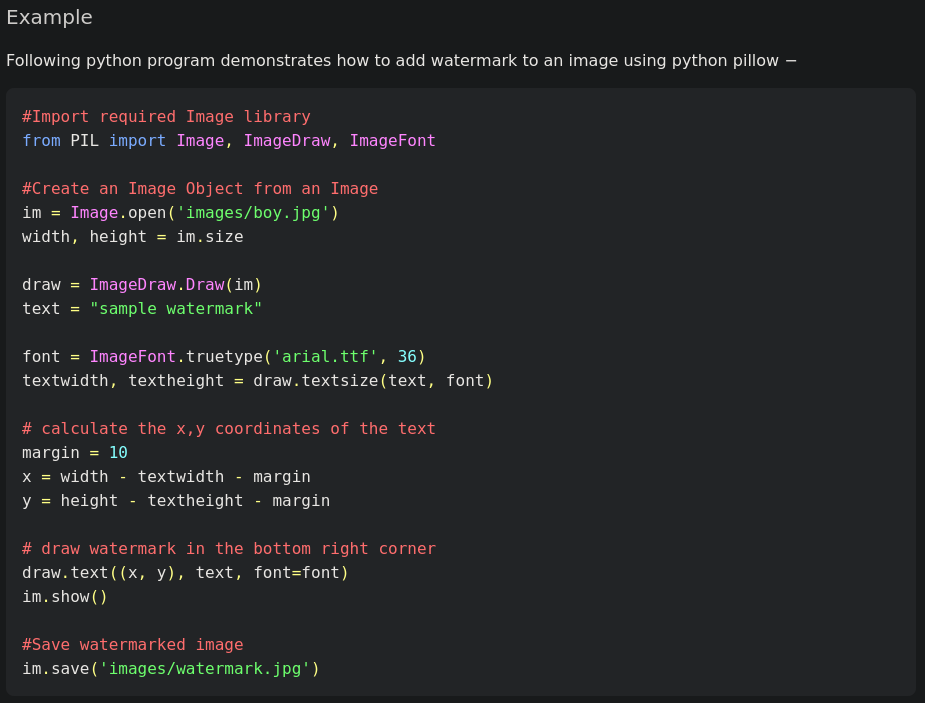
\includegraphics[width=\linewidth]{img/website1.png}
		\end{figure}
	\end{columns}
\end{frame}

\begin{frame}{Wasserzeichen}
	\begin{figure}[H]
		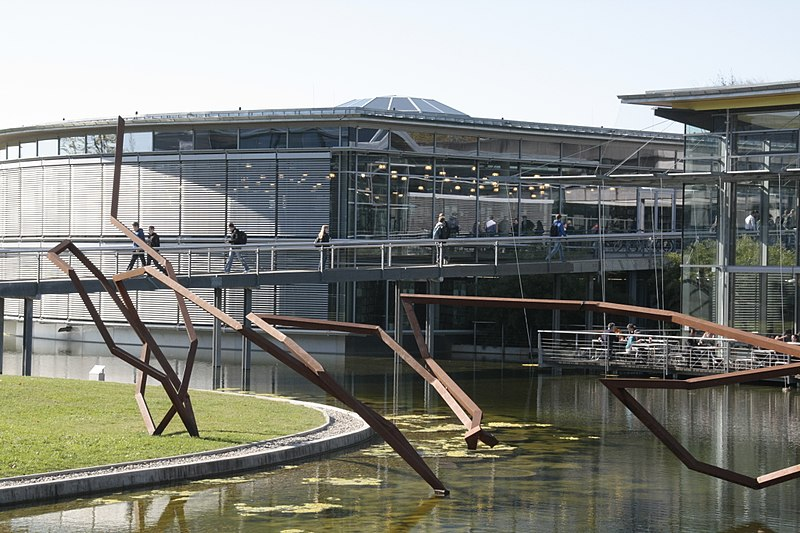
\includegraphics[height=0.8\textheight]{img/oth.jpg}
	\end{figure}
\end{frame}

\begin{frame}{Wasserzeichen}
	\begin{figure}[H]
		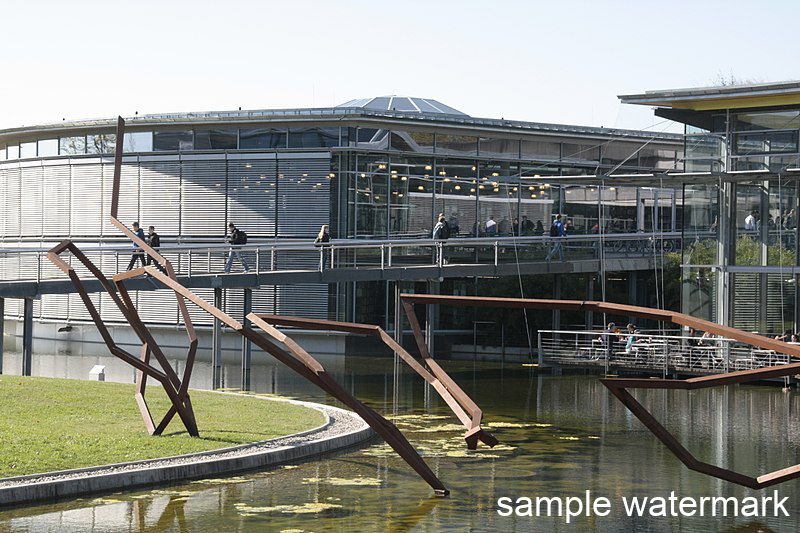
\includegraphics[height=0.8\textheight]{img/oth-wm.png}
	\end{figure}
\end{frame}

\begin{frame}{Wasserzeichen}
	\begin{figure}[H]
		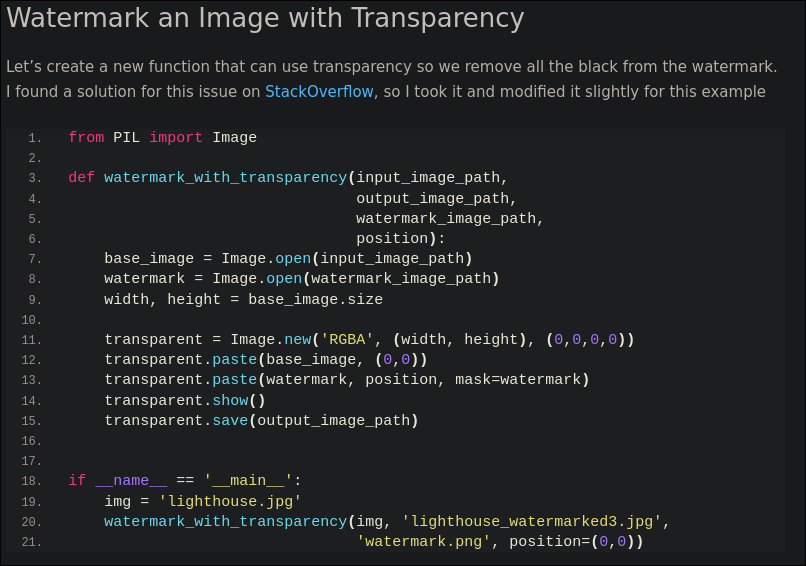
\includegraphics[height=0.8\textheight]{img/website2.png}
	\end{figure}
\end{frame}

\subsection{fertiges Wasserzeichen}
\begin{frame}{fertiges Wasserzeichen}
	\begin{figure}[H]
		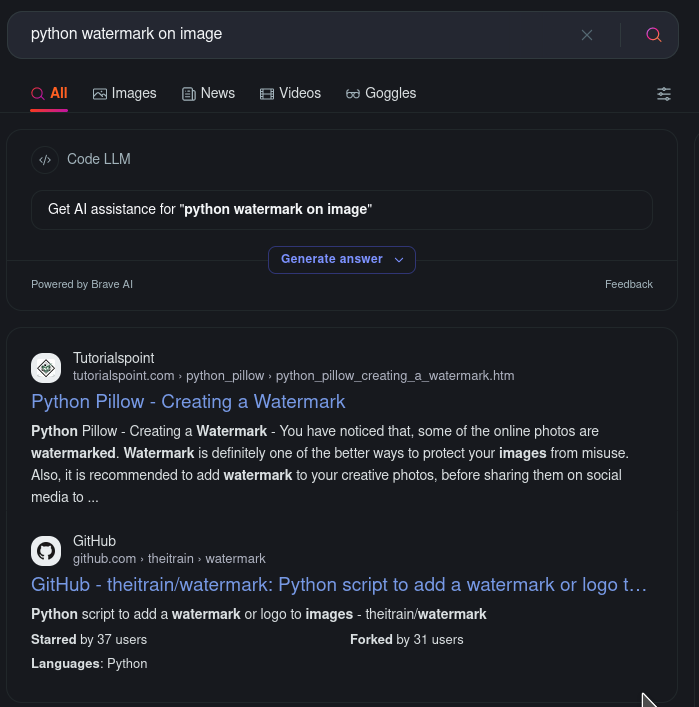
\includegraphics[height=0.8\textheight]{img/first-search.png}
	\end{figure}
\end{frame}

\begin{frame}
\end{frame}

\begin{frame}{Quellen}
	% TODO update letzter Zugriff
	\begin{thebibliography}{99}
		{\fontfamily{lucida}\selectfont\small
			\bibitem{search} \textit{https://search.brave.com}. letzter Zugriff 2024/17/04.
			\bibitem{first_website} \textit{https://www.tutorialspoint.com/python\_pillow/python\_pillow\_creating\_a\_ \\ \ \ \ \ watermark.htm}. letzter Zugriff 2024/17/04.
			\bibitem{oth} \textit{https://de.wikipedia.org/wiki/Ostbayerische\_Technische\_Hochschule\_ \\ \ \ \ \ Regensburg}. letzter Zugriff 2024/17/04.
			\bibitem{second_website} \textit{https://www.blog.pythonlibrary.org/2017/10/17/how-to-watermark-\\ \ \ \ \ your-photos-with-python}. letzter Zugriff 2024/17/04.
			\bibitem{chatgpt} \textit{https://chat.openai.com}. letzter Zugriff 2024/17/04.
		}
	\end{thebibliography}
\end{frame}

\end{document}
